\documentclass[]{article}

% Imported Packages
%------------------------------------------------------------------------------
\usepackage{amssymb}
\usepackage{amstext}
\usepackage{amsthm}
\usepackage{amsmath}
\usepackage{enumerate}
\usepackage{fancyhdr}
\usepackage[margin=1in]{geometry}
\usepackage{graphicx}
\usepackage{extarrows}
\usepackage{setspace}
%------------------------------------------------------------------------------

% Header and Footer
%------------------------------------------------------------------------------
\pagestyle{plain}  
\renewcommand\headrulewidth{0.4pt}                                      
\renewcommand\footrulewidth{0.4pt}                                    
%------------------------------------------------------------------------------


% Title Details
%------------------------------------------------------------------------------
\title{Deliverable \#2}
\author{Group \#4 \\
Attia, Abrar - attiaa1 - 400017188 \\
Ansell, Evan - ansellea - 1415992 \\
Fayez, Susan - fayezs - 001404420 \\
Yin, Hao - yinh1 - 400016540 \\
Yang, Zhiwen - yangz18 - 400023048 }
\date{2018-03-09}                               
%------------------------------------------------------------------------------
 
% Document
%------------------------------------------------------------------------------
\begin{document}

\maketitle	
\newpage

\section{Introduction}
\label{sec:introduction}
% Begin Section



\subsection{Purpose}
\label{sub:purpose}
The purpose of this document is to provide a thorough description of the whole system with different kinds of system diagrams. The document will also include a summary on the architecture design of the system. In addition, the following document will be used to build and develop the classes required for the Forester application. The intended audience of the document is mainly the software developers and project managers.

\subsection{System Description}
\label{sub:system_description}

The Forester system is a plant identification system implemented by Blackboard Architecture. It accepts three user types: average users, researchers and administrators. They have different levels of permission to view and manipulate data from the data source. The system stores plant data and identifies designated matches according to the input of users. The users enter a number of different plant characteristics which are checked by the relevant experts. Then the system fetches data from the data source and displays output to the users. \\
	\\
The whole system contains four entities(Plant Data, Search History, Registered Users, Modifications) which hold all the data of the system. With the help of controller classes(I/O Controller, Identification Experts, Security, Modification Controller), users are able to login, edit account information, send input, receive output and edit plant data. The system also consists of eleven boundary classes: Identify Plant, Results, View Search History, View Data, Login, Login Error, Change Password, Submit Modifications, Manage Modifications, Researcher and Administrator. They communicate with entity classes by controllers to realize data transmission back and forth.

\subsection{Overview}
\label{sub:overview}
The remaining sections of the document contains two different system diagrams which are the use case diagram and the analysis class diagram. The overall architectural design of the application is also discussed later on and focuses on two aspects which are the system architecture and the subsystems. This is then followed by class responsibility collaboration cards for the boundary classes, control classes, and entity classes. The document then ends with a division of labour sheet.

% End Section


\section{Use Case Diagram}
\label{sec:use_case_diagram}
% Begin Section
\begin{enumerate}[1.]
	\item The User wants to identify a plant. They can either answer the ID questions to identify a specific plant or enter a location to identify the plants native to that area. The system produces the results.
	\item The User wants to view the results of a past search, the system displays it.
	\item The User wants to clear their search history. The system prompts them to confirm the deletion.
	\item The Rearcher or the Administrator wants to log in to the system. The system validtates their credentials.
	\item The Researcher wants to view the database. The system displays it.
	\item The Researcher wants to submit a Database Update Request. The type of request can be either an Edit, Addition, or Deletion.
	\item The Researcher wants to view their contributions. The system displays them.
	\item The Researcher or the Administrator wants to update their password. The system prompts them to confirm the update.
	\item The Administrator wants to manage the Database Update Requests. They can either display the requests, confirm requests, or deny requests.
\end{enumerate}

    \begin{figure}[!hb]
      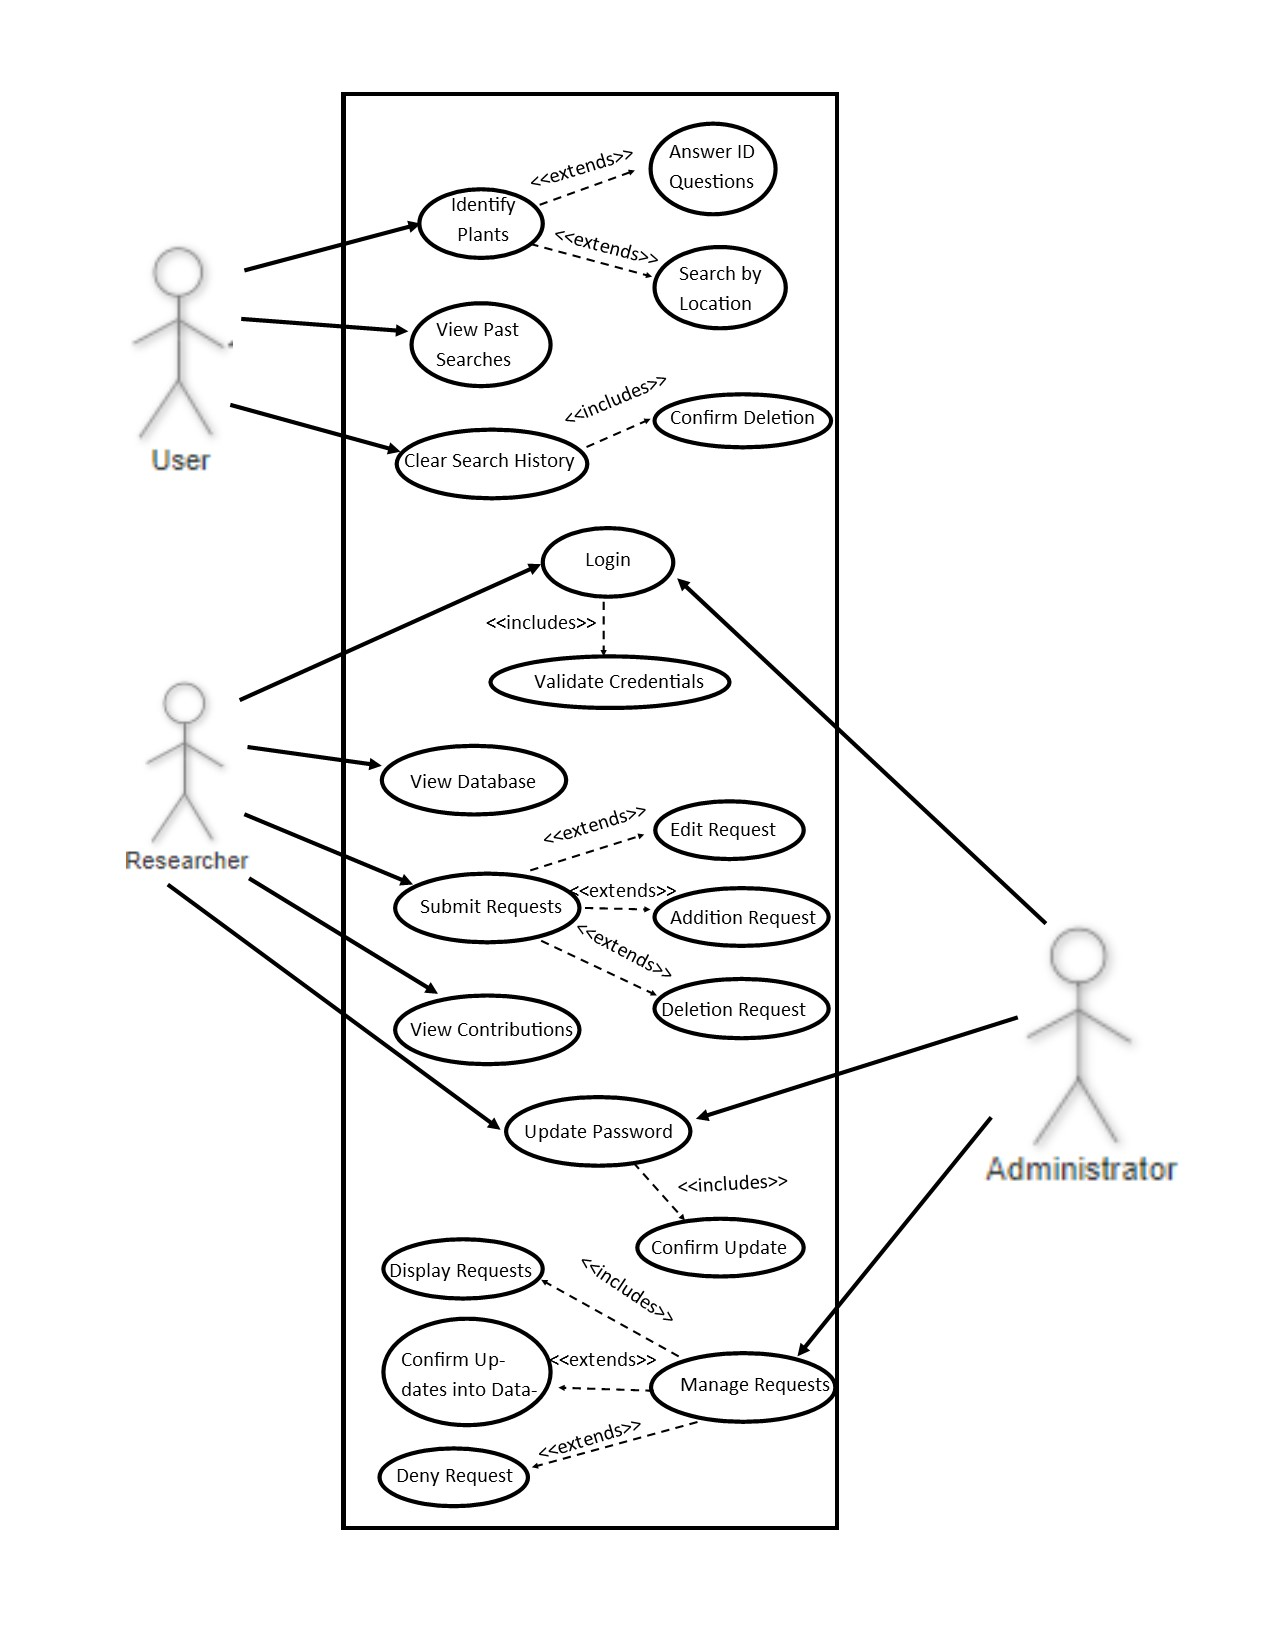
\includegraphics[width=\linewidth]{usecase.jpg}
      \caption{Use Case Diagram}
      \label{fig:UCD}
    \end{figure}
    
    Figure \ref{fig:UCD} displays the Use Case Diagram for the Forester system.

\clearpage
% End Section

\section{Analysis Class Diagram}
\label{sec:analysis_class_diagram}
% Begin Section

    \begin{figure}[!hb]
      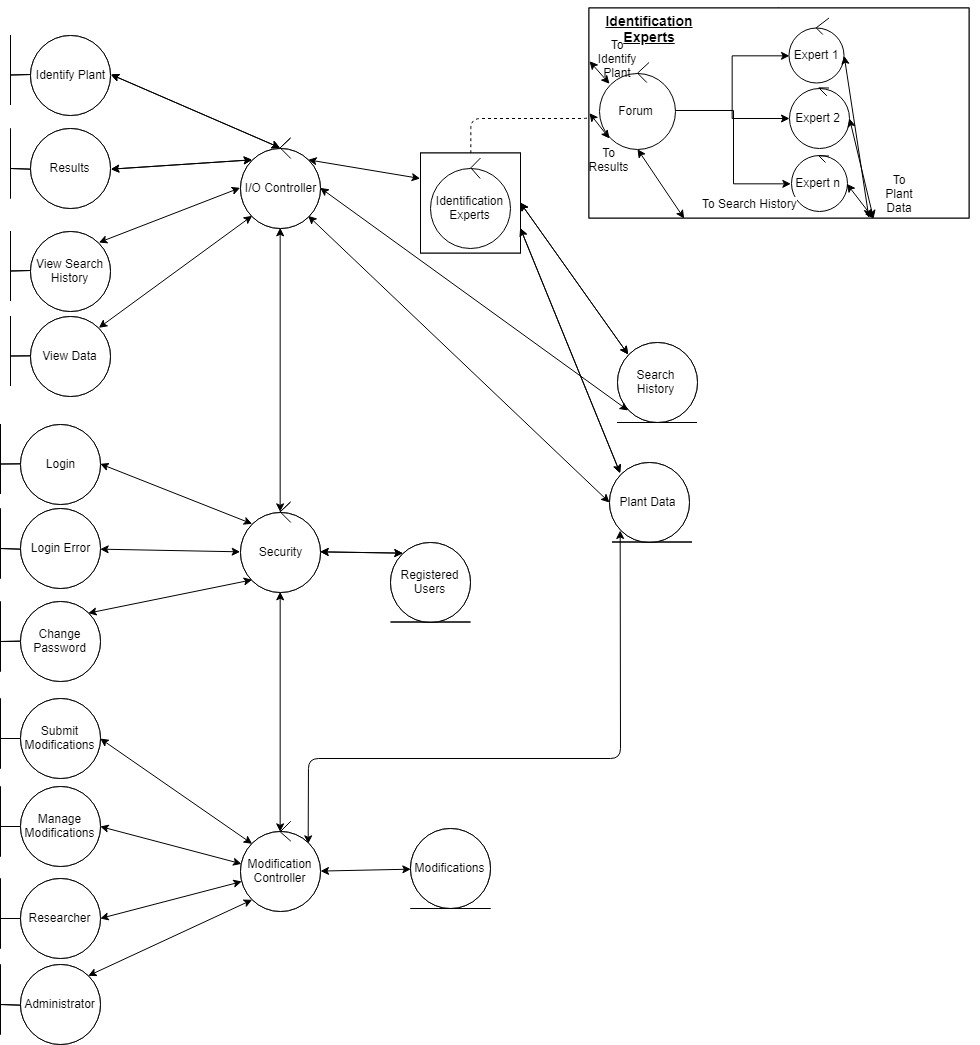
\includegraphics[width=\linewidth]{ACD.jpg}
      \caption{Analysis Class Diagram}
      \label{fig:ACD}
    \end{figure}
    
% End Section
\clearpage

\section{Architectural Design}
\label{sec:architectural_design}
% Begin Section

\subsection{System Architecture}
\label{sub:system_architecture}
% Begin SubSection
	 The overall architecture of the Forester system is Blackboard Architecture. To begin, the main functionality of the system is to identify plants based on specified characteristics. These characteristics are entered by the user as observations and the blackboard system is used to compare the observations to the data facts which exist in the expert specialists. In addition, Forester is mainly a blackboard architecture since each expert acts as a knowledge source and works independently from one another. Each expert provides a partial solution to what plant has been described and a final solution is determined by combining the results of each knowledge source. Moreover, the plant data class would act as the data store in the architecture which further justifies the choice of blackboard architecture for the system. The Forester system also includes other subsystems that may be excluded from the blackboard architecture; however, they are very minor in comparison to the core functionality of the system which is to use experts to identify plants based on inputted specifications.\\
	 Below is a Structural Architecture Diagram of the system which assists in understanding why the overall architecture of the system is a blackboard architecture. The blue box of the analysis class diagram is identified as the Identification subsystem which features all the classes that are attributed to the blackboard architecture. The remaining subsystems are much more minor in comparison to the Identification subsystem and do not have a large impact on the overall architecture.
	
    \begin{figure}
      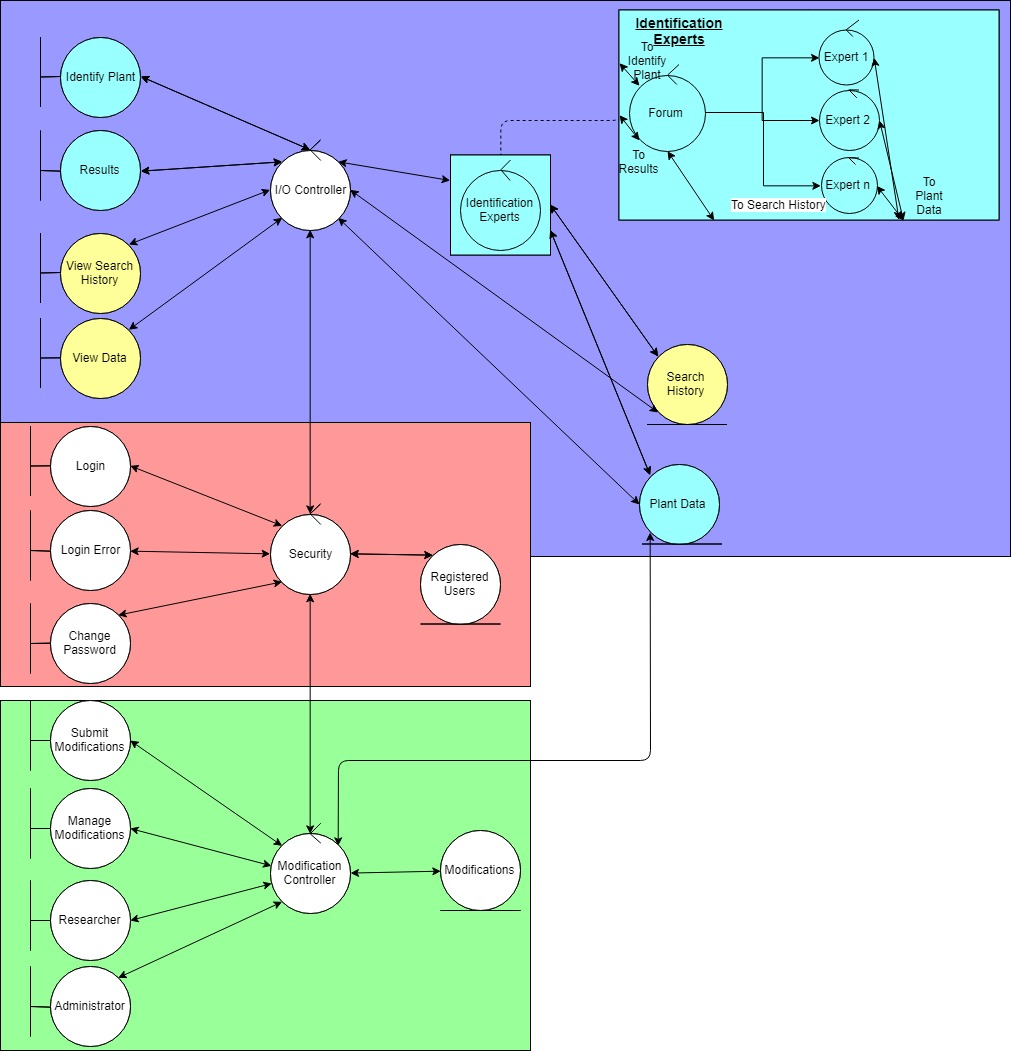
\includegraphics[width=\linewidth]{subsystems.jpg}
      \caption{Structural Architecture Diagram - Subsystems}
      \label{fig:SAD1}
    \end{figure}
    
    Figure \ref{fig:SAD1} shows the different subsystems within Forester.

% End SubSection

\subsection{Subsystems}
\label{sub:subsystems}
% Begin SubSection

The subsystems of Forester are displayed in Figure 1 - Structural Architecture Diagram. As shown, the Forester system is divided into 3 major subsystems with the largest being the Identification subsystem (blue box). The identification subsystem deals with the main functionality of the application which is to allow users to identify plants based on inputted characteristics and comparing them to the experts in order to produce a result, as well as viewing search history and data. This subsystem is then divided into 2 smaller subsystems which include the Identification Agents subsystem (light blue classes) and the Data Retention and Searching subsystem (yellow classes). The Identification Agents subsystem features the classes that take user input, analyze it using the experts, and return a result. Whereas, the Data Retention and Searching subsystem focuses on allowing the user to view their past searches and the data on file. In addition, another subsystem of Forester is the Authentication subsystem (pink box) which focuses on the system security and user login operations. The last subsystem is the High Level Modification subsystem (green box) which controls the abilities of different types of users including the researchers and the administration. The researchers and admin need to be approved by the security controller in the Authentication subsystem in order to move onto the High Level Modification subsystem and to make alterations to the plant data. Moreover, the Authentication subsystem works alongside the Identification subsystem and the High Level Modification subsystem by allowing users to login and gain access to the different functions of the application. 
\clearpage
% End SubSection

% End Section
	
\section{Class Responsibility Collaboration (CRC) Cards}
\label{sec:class_responsibility_collaboration_crc_cards}
\subsection{Boundary Classes}
% Begin Section
%	\begin{table}[ht]
		\centering
		\begin{tabular}{|p{7cm}|p{7cm}|}
		\hline 
		 \multicolumn{2}{|l|}{\textbf{Class Name: Identify Plant}} \\
		\hline
		\textbf{Responsibility:} & \textbf{Collaborators:} \\
		\hline
		\text{Receive user input} & \text{}\\
		\hline
		\text{Send input data to experts} & \text{I/O Controller} \\
		\hline
		Send location data to experts & I/O Controller\\
		\hline
		\text{Begin login process} & \text{I/O Controller}\\
		\hline
		\end{tabular}
%	\end{table}
	\newline
	\vspace*{0.5 cm}
	\newline
%\begin{table}[ht]
		\centering
		\begin{tabular}{|p{7cm}|p{7cm}|}
		\hline 
		 \multicolumn{2}{|l|}{\textbf{Class Name: Results}} \\
		\hline
		\textbf{Responsibility:} & \textbf{Collaborators:} \\
		\hline
		\text{Receive result data from experts} & \text{I/O Controller}\\
		\hline
		\text{Display result} & \text{}\\
		\hline
		Return to Identify Plant page & I/O Controller\\
		\hline
		\end{tabular}
%	\end{table}
	\newline
	\vspace*{0.5 cm}
	\newline
%\begin{table}[ht]
		\centering
		\begin{tabular}{|p{7cm}|p{7cm}|}
		\hline 
		 \multicolumn{2}{|l|}{\textbf{Class Name: View Search History}} \\
		\hline
		\textbf{Responsibility:} & \textbf{Collaborators:} \\
		\hline
		Request search data & I/O Controller\\
		\hline
		Display search history & \\
		\hline
		Sort and filter displayed data & I/O Controller\\
		\hline
		Return to Identify Plant page & I/O Controller\\
		\hline
		\end{tabular}
%	\end{table}
	\newline
	\vspace*{0.5 cm}
	\newline

%\begin{table}[ht]
		\centering
		\begin{tabular}{|p{7cm}|p{7cm}|}
		\hline 
		 \multicolumn{2}{|l|}{\textbf{Class Name: View Data}} \\
		\hline
		Request plant data & I/O Controller\\
		\hline
		Display plant data & \\
		\hline
		Sort and filter displayed data & I/O Controller\\
		\hline
		Return to Researcher page & I/O Controller\\
		\hline
		\end{tabular}
%	\end{table}
	\newline
	\vspace*{0.5 cm}
	\newline

%\begin{table}[ht]
		\centering
		\begin{tabular}{|p{7cm}|p{7cm}|}
		\hline 
		 \multicolumn{2}{|l|}{\textbf{Class Name: Login}} \\
		\hline
		\textbf{Responsibility:} & \textbf{Collaborators:} \\
		\hline
		Receive user input & \\
		\hline
		Send input data to Security controller for validation & Security\\
		\hline
		Return to Identify Plant & Security\\
		\hline
		\end{tabular}
%	\end{table}
	\newline
	\vspace*{0.5 cm}
	\newline
%\begin{table}[ht]
		\centering
		\begin{tabular}{|p{7cm}|p{7cm}|}
		\hline 
		 \multicolumn{2}{|l|}{\textbf{Class Name: Login Error}} \\
		\hline
		\textbf{Responsibility:} & \textbf{Collaborators:} \\
		\hline
		Display error message & \\
		\hline		
		Rreturn to Login & Security\\
		\hline
		Return to Identify Plant & Security\\
		\hline
		\end{tabular}
%	\end{table}
	\newline
	\vspace*{0.5 cm}
	\newline


%\begin{table}[ht]
		\centering
		\begin{tabular}{|p{7cm}|p{7cm}|}
		\hline 
		 \multicolumn{2}{|l|}{\textbf{Class Name: Change Password}} \\
		\hline
		\textbf{Responsibility:} & \textbf{Collaborators:} \\
		\hline
		Receive user input (password) & \\
		\hline
		Send input data to Security controller & Security \\
		\hline
		Return to previous page (Researcher or Administrator) & Security \\
		\hline
		\end{tabular}
%	\end{table}
	\newline
	\vspace*{0.5 cm}
	\newline
%\begin{table}[ht]
		\centering
		\begin{tabular}{|p{7cm}|p{7cm}|}
		\hline 
		 \multicolumn{2}{|l|}{\textbf{Class Name: Submit Modifications}} \\
		\hline
		\textbf{Responsibility:} & \textbf{Collaborators:} \\
		\hline
		Receive user input & \\
		\hline
		Send user input to Modification Controller  & Modification Controller \\
		\hline
		Return to Researcher page & Modification Controller \\
		\hline
		\end{tabular}
%	\end{table}
	\newline
	\vspace*{0.5 cm}
	\newline
%\begin{table}[ht]
		\centering
		\begin{tabular}{|p{7cm}|p{7cm}|}
		\hline 
		 \multicolumn{2}{|l|}{\textbf{Class Name: Manage Modifications}} \\
		\hline
		\textbf{Responsibility:} & \textbf{Collaborators:} \\
		\hline
		Request Modification data & Modification Controller \\
		\hline
		Display Modification date & \\
		\hline
		Write modified data to main Plant Data & Modification Controller \\
		\hline
		Return to Administrator page & Modification Controller \\
		\hline
		\end{tabular}
%	\end{table}
	\newline
	\vspace*{0.5 cm}
	\newline

%\begin{table}[ht]
		\centering
		\begin{tabular}{|p{7cm}|p{7cm}|}
		\hline 
		 \multicolumn{2}{|l|}{\textbf{Class Name: Researcher}} \\
		\hline
		\textbf{Responsibility:} & \textbf{Collaborators:} \\
		\hline
		View data & Modification controller \\
		\hline
		Request modifications &  Modification controller \\
		\hline
		Change password &  Modification controller \\
		\hline
		Log out and return to Login page &  Modification controller\\
		\hline
		\end{tabular}
%	\end{table}
	\newline
	\vspace*{0.5 cm}
	\newline

%\begin{table}[ht]
		\centering
		\begin{tabular}{|p{7cm}|p{7cm}|}
		\hline 
		 \multicolumn{2}{|l|}{\textbf{Class Name: Administrator}} \\
		\hline
		\textbf{Responsibility:} & \textbf{Collaborators:} \\
		\hline
		Manage modifications & Modification controller \\
		\hline
		Change password &  Modification controller \\
		\hline
		Log out and return to Login page &  Modification controller\\
		\hline
		\end{tabular}
%	\end{table}
	\newline
	\vspace*{0.5 cm}
	\newline

\subsection{Controller Classes}

%\begin{table}[ht]
		\centering
		\begin{tabular}{|p{7cm}|p{7cm}|}
		\hline 
		 \multicolumn{2}{|l|}{\textbf{Class Name: I/O Controller}} \\
		\hline
		\textbf{Responsibility:} & \textbf{Collaborators:} \\
		\hline
		Accept plant data from Identify Plant & Identify Plant \\
		\hline
		Send plant data to Identification Experts & Forum \\
		\hline
		Accept plant result data from Identification Experts & Forum \\
		\hline
		Send plant results from the Identification Experts to Results and open the Results page & Results \\
		\hline
		Receive sort and filter data & View Search History, View Data \\
		\hline
		Read search history data & Search History \\
		\hline
		Read plant data & Plant Data \\
		\hline
		Modify history or plant data based on specified sort and filters & \\
		\hline
		Receive request for Identify Plant page and open it & Security, Results, View Search History, Identify Plant \\
		\hline
		Receive request for Search History page and open it & Security, View Search History \\
		\hline
		Receive request for View Data page and open it & Security, View Data \\
		\hline
		Request for Login page to be opened & Security \\
		\hline
		Request for Researcher page to be opened & Security \\
		\hline
		\end{tabular}
%	\end{table}
	\newline
	\vspace*{0.5 cm}
	\newline

%\begin{table}[ht]
		\centering
		\begin{tabular}{|p{7cm}|p{7cm}|}
		\hline 
		 \multicolumn{2}{|l|}{\textbf{Class Name: Security}} \\
		\hline
		\textbf{Responsibility:} & \textbf{Collaborators:} \\
		\hline
		\text{Receive username and password} & \text{Login} \\
		\hline
		\text{Access registered data} & \text{Registered Users} \\
		\hline
		\text{Search for username} & \text{Registered Users} \\
		\hline
		\text{Validate password} & \text{Registered Users} \\
		\hline
		\text Open Login Error page if username/password incorrect & \text{Login Error} \\
		\hline
		Accept new password for current user & Change Password \\
		\hline
		Write new password to Registered Users for current user & Registered Users \\
		\hline
		Receive request for Login page and open it & I/O Controller, Modification Controller, Login Error, Login  \\
		\hline
		Receive request for Change Password page and open it & Modification Controller, Change Password \\
		\hline
		Relay request for View Data page to be opened & Modification Controller, I/O Controller \\
		\hline
		Relay request for Researcher page to be opened & I/O Controller, Modification Controller \\
		\hline
		Request for Researcher page to be opened when a researcher logs in & \text{Modification Controller} \\
		\hline
		Request for Administrator page to be opened when an administrator logs in & \text{Modification Controller} \\
		\hline
		\end{tabular}
%	\end{table}
	\newline
	\vspace*{0.5 cm}
	\newline

%\begin{table}[ht]
		\centering
		\begin{tabular}{|p{7cm}|p{7cm}|}
		\hline 
		 \multicolumn{2}{|l|}{\textbf{Class Name: Modification Controller}} \\
		\hline
		\textbf{Responsibility:} & \textbf{Collaborators:} \\
		\hline
		Receive modification data & Submit Modifications \\
		\hline
		Write modification data & Modifications \\
		\hline
		Receive request for data of current modifications & Manage Modifications \\
		\hline
		Read modification data & Modifications \\
		\hline
		Send modification data to Manage Modifications & Manage Modifications \\
		\hline
		Receive request to merge current modifications into Plant Data & Manage Modifications \\
		\hline 
		Write modification data to Plant Data & Plant Data \\
		\hline
		Receive request for Researcher page and open it & Security, Researcher \\
		\hline
		Receive request for Administrator page and open it & Security, Administrator\\
		\hline
		Receive request for Submit Modifications page and open it &  Researcher, Submit Modifications \\
		\hline
		Receive request for Manage Modifications page and open it & Administrator, Manage Modifications \\
		\hline
		Request for Login page to be opened & Researcher, Administrator, Security \\
		\hline
		Request for View Data page to be opened & Researcher, Security \\
		\hline
		\end{tabular}
%	\end{table}
	\newline
	\vspace*{0.5 cm}
	\newline

%\begin{table}[ht]
		\centering
		\begin{tabular}{|p{7cm}|p{7cm}|}
		\hline 
		 \multicolumn{2}{|l|}{\textbf{Class Name: Forum}} \\
		\hline
		\textbf{Responsibility:} & \textbf{Collaborators:} \\
		\hline
		\text{Receive plant data} & \text{I/O Controller} \\
		\hline
		\text{Send plant data to relevant experts} & \text{Expert} \\
		\hline
		Send plant data search to Search History & Search history \\
		\hline
		Receive results from each expert & Expert \\
		\hline
		Determine the best result based on the experts' results & \\
		\hline
		Send the best result to Results & I/O Controller \\
		\hline
		If only location data given from user, send all results from the location-only expert to Results & I/O Controller \\
		\hline
		Send error result & I/O Controller \\
		\hline
		\end{tabular}
%	\end{table}
	\newline
	\vspace*{0.5 cm}
	\newline

%\begin{table}[ht]
		\centering
		\begin{tabular}{|p{7cm}|p{7cm}|}
		\hline 
		 \multicolumn{2}{|l|}{\textbf{Class Name: Expert}} \\
		\hline
		\textbf{Responsibility:} & \textbf{Collaborators:} \\
		\hline
		\text{Receive plant data} & \text{Forum} \\
		\hline
		\text{Access plant data} & \text{Plant Data} \\
		\hline
		\text{Search through plant data} & \text{Plant Data} \\
		\hline
		\text{Return plants matching given plant data} & \text{Forum} \\
		\hline
		\end{tabular}
%	\end{table}
	\newline
	\vspace*{0.5 cm}
	\newline


\subsection{Entity Classes}
	%\begin{table}[ht]
		\centering
		\begin{tabular}{|p{7cm}|p{7cm}|}
		\hline 
		 \multicolumn{2}{|l|}{\textbf{Class Name: Plant Data}} \\
		\hline
		\textbf{Responsibility:} & \textbf{Collaborators:} \\
		\hline
		Hold plant data & \\
		\hline
		Provide read access to plant data & Expert, I/O Controller \\
		\hline
		Provide write access to plant data & Modification Controller \\
		\hline
		\end{tabular}
%	\end{table}
	\newline
	\vspace*{0.5 cm}
	\newline

%\begin{table}[ht]
		\centering
		\begin{tabular}{|p{7cm}|p{7cm}|}
		\hline 
		 \multicolumn{2}{|l|}{\textbf{Class Name: Search History}} \\
		\hline
		\textbf{Responsibility:} & \text{Collaborators:} \\
		\hline
		Hold search history data & \\
		\hline
		Provide read access to search data & I/O Controller \\
		\hline
		Provide write access to search data & Forum \\
		\hline
		\end{tabular}
%	\end{table}
	\newline
	\vspace*{0.5 cm}
	\newline

%\begin{table}[ht]
		\centering
		\begin{tabular}{|p{7cm}|p{7cm}|}
		\hline 
		 \multicolumn{2}{|l|}{\textbf{Class Name: Registered Users}} \\
		\hline
		\textbf{Responsibility:} & \text{Collaborators:} \\
		\hline
		Hold username, password, and classification of users & \\
		\hline
		Provide read access to user data & Security \\
		\hline
		Provide write access to user data & Security \\
		\hline
		\end{tabular}
%	\end{table}
	\newline
	\vspace*{0.5 cm}
	\newline

%\begin{table}[ht]
		\centering
		\begin{tabular}{|p{7cm}|p{7cm}|}
		\hline 
		 \multicolumn{2}{|l|}{\textbf{Class Name: Modifications}} \\
		\hline
		\textbf{Responsibility:} & \text{Collaborators:} \\
		\hline
		Hold data of modifications to be made to plant data & \\
		\hline
		Provide read access to modification data & Modification Controller \\
		\hline 
		Provide write access modification data & Modification controller \\
		\hline
		\end{tabular}
%	\end{table}
	\newline
	\vspace*{0.5 cm}
	\newline

\newpage
\appendix
\section{Division of Labour}
\label{sec:division_of_labour}
% Begin Section

Purpose - Allen\\
System Description - Hao \\
Overview - Allen\\
Use Case Diagram - Susan\\
Analysis Class Diagram - Evan, Hao, Abrar\\
System Architecture - Abrar \\
Subsystems - Abrar\\
CRC cards - Everyone (Evan)\\
Division of Labour - Abrar\\

% End Section



\end{document}
%------------------------------------------------------------------------------
